\chapter{Contextual and Spatial Information in V1 Responses}
\label{chapterlabel4}
In previous chapter, the mice behaviour validates that mice can learn a complex visual navigation task with identical landmarks and can distinguish the two visual environments with identical landmarks at various positions and contexts. As described in chapter 2, the neuropixel recordings in V1 provide a rich dataset in how V1 neurons respond to visual landmarks in the dynamically changing environments. In previous study, spatial modulation is present when animal travels in a VR designed similar as the familiar environment used in training and the spatial modulation is stronger over days of contact with the VR environment. In the recordings, a novel environment is introduced with new sets of identical landmarks at same locations but also with a set of plaid landmarks shared between the familiar and novel environments. This chapter aims to characterise the V1 responses in the two spatial contexts by first replicating the spatial modulation found in V1 and exploring if spatial context has impact on visual responses in V1.



\section{V1 Neurons Have Diverse Tuning to the Visual Features in VR}

\begin{figure}
    \centering
    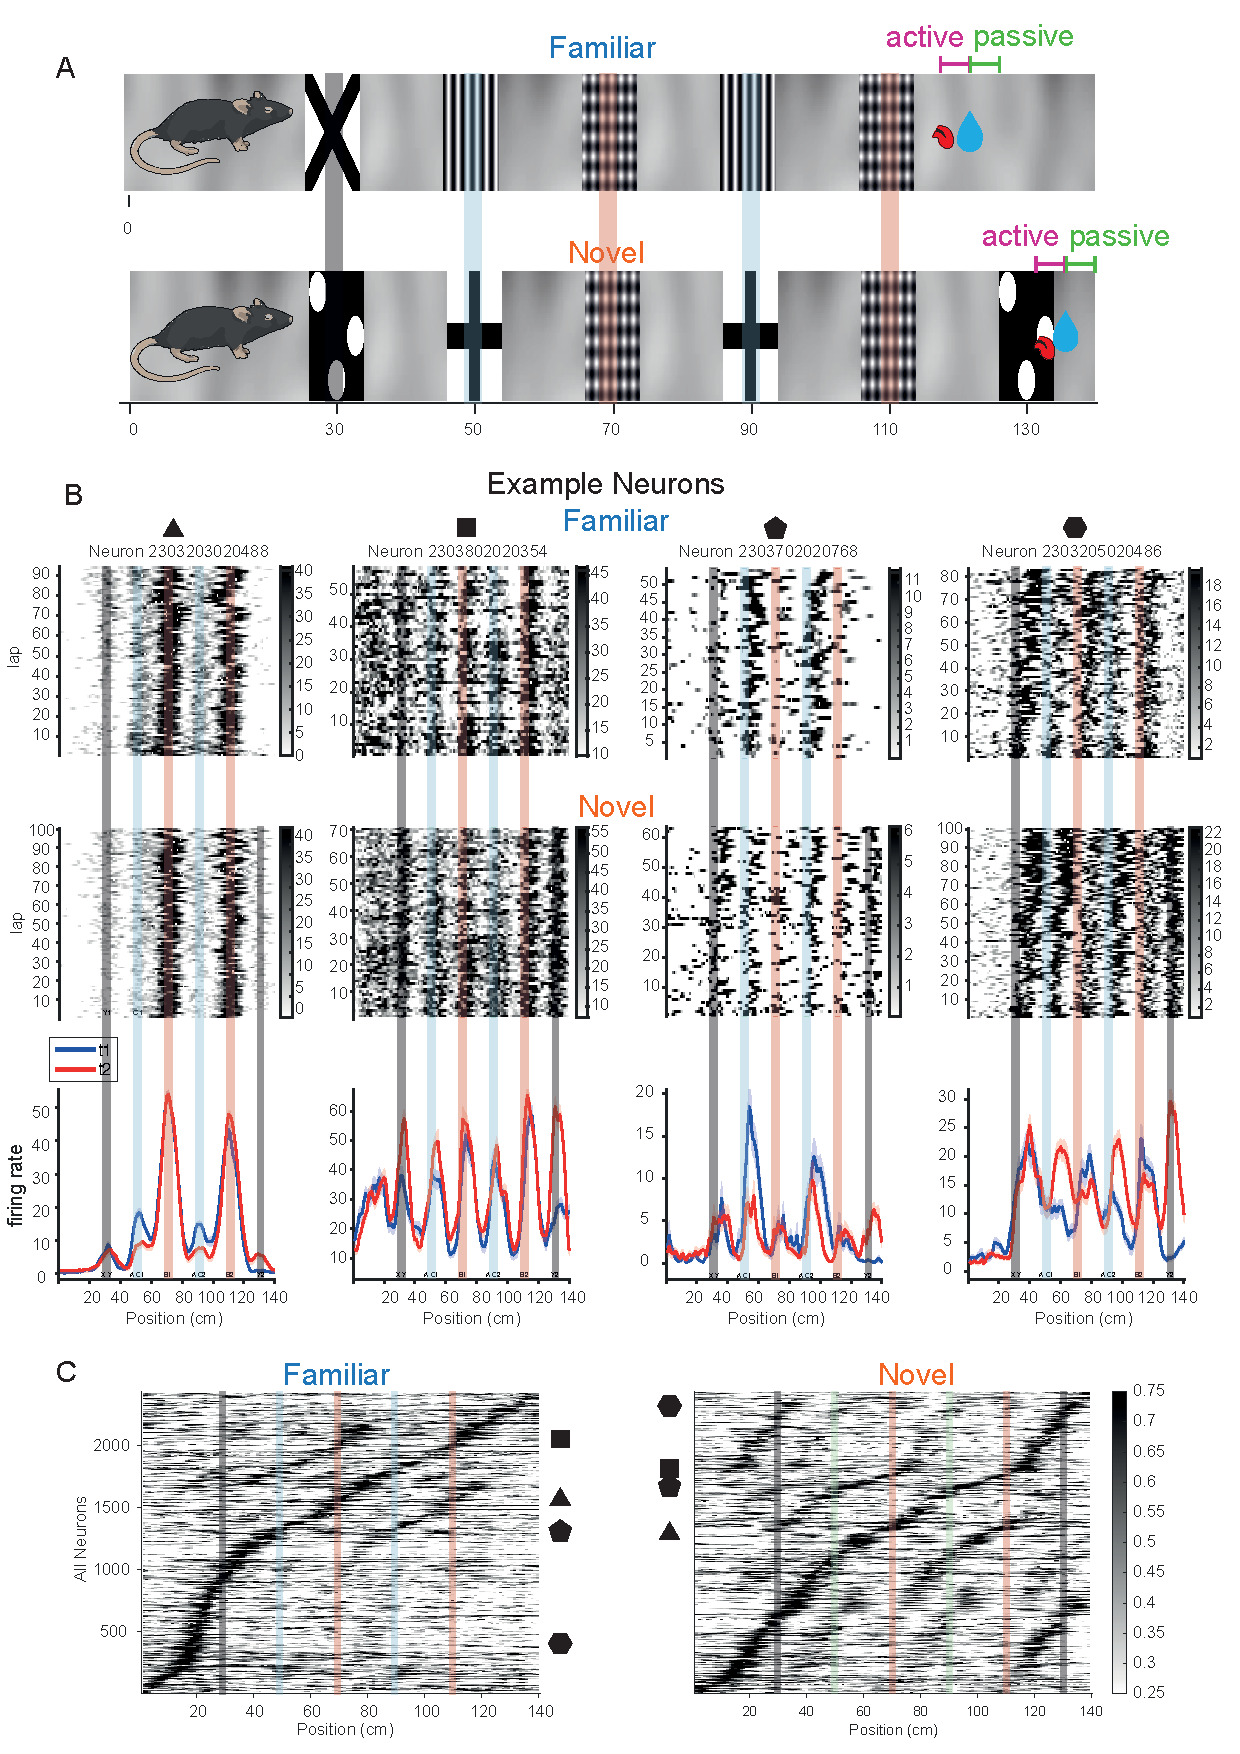
\includegraphics[width=1\linewidth]{figures//Chapter 4 V1/fig1_VR_setup_and_responses.pdf}
    \caption{A summary of visual responses in the two VR environments sorted by position and examples neurons' tuning PSTH.}
    \label{fig:population map}
\end{figure}




\begin{figure}
    \centering
    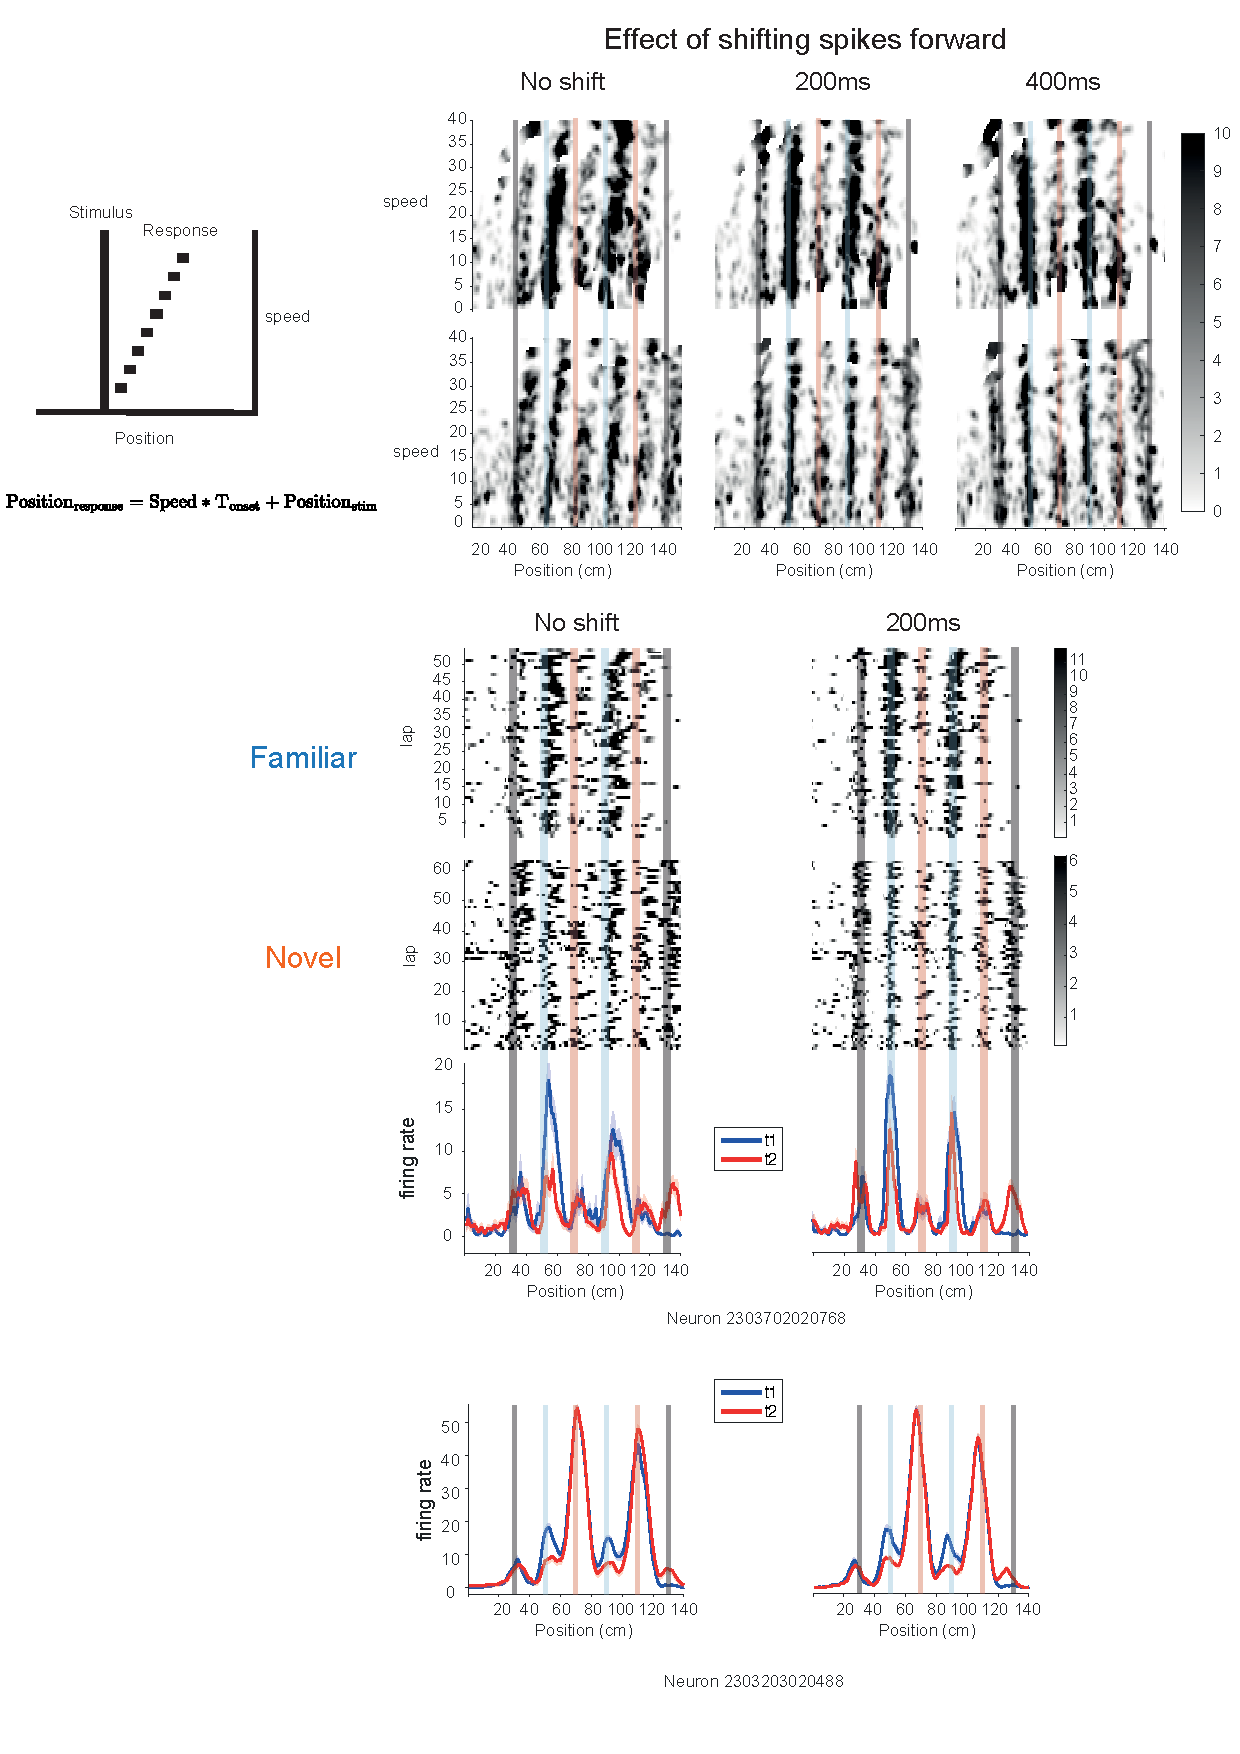
\includegraphics[width=1\linewidth]{figures//Chapter 4 V1/fig2_speed_impact.pdf}
    \caption{Visual cortical responses have delays and their impact on spatial binning depends on the animal's speed in the VR. }
    \label{fig:placeholder}
\end{figure}


\begin{figure}
    \centering
    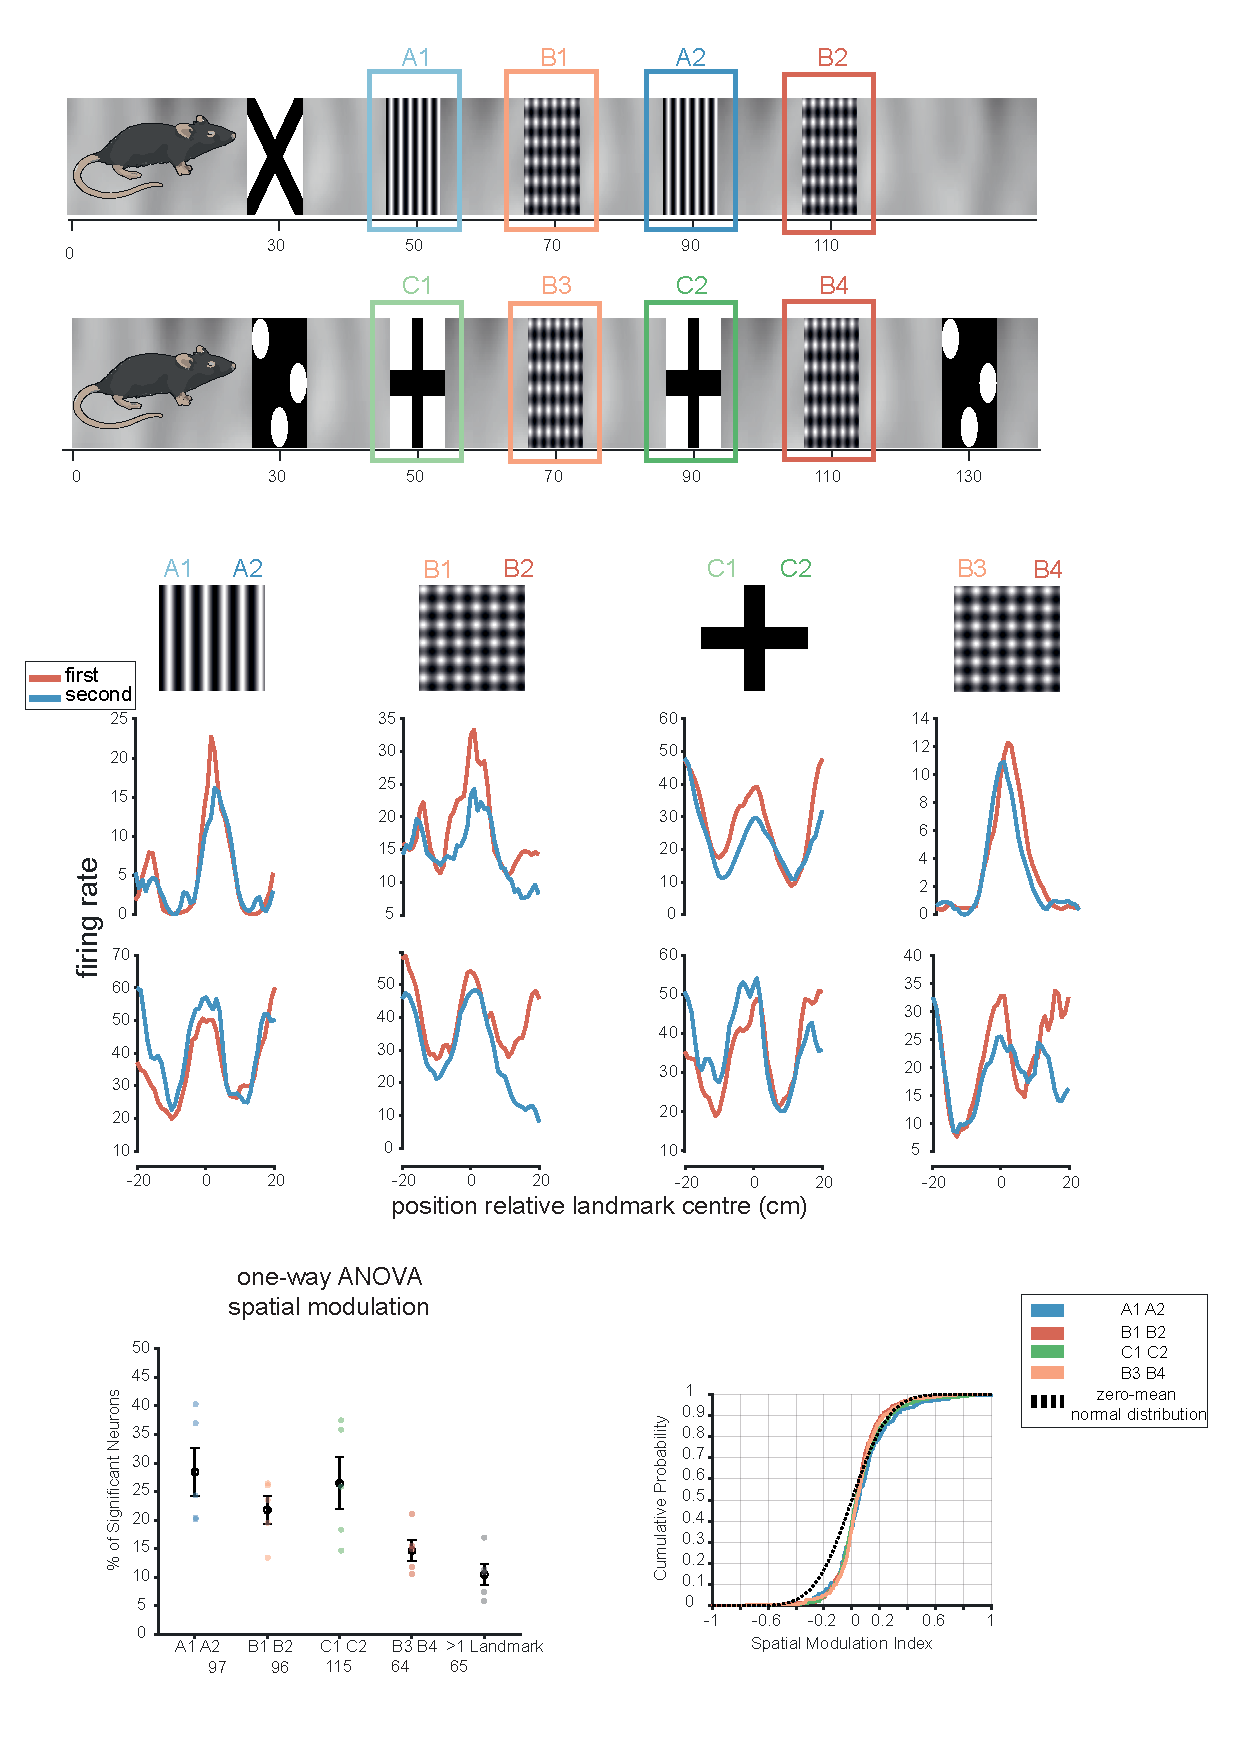
\includegraphics[width=1\linewidth]{figures//Chapter 4 V1/fig3_spatial_modulation_intro.pdf}
    \caption{Spatial modulation on landmark-specific responses in both environments}
    \label{fig:placeholder}
\end{figure}


\begin{figure}
    \centering
    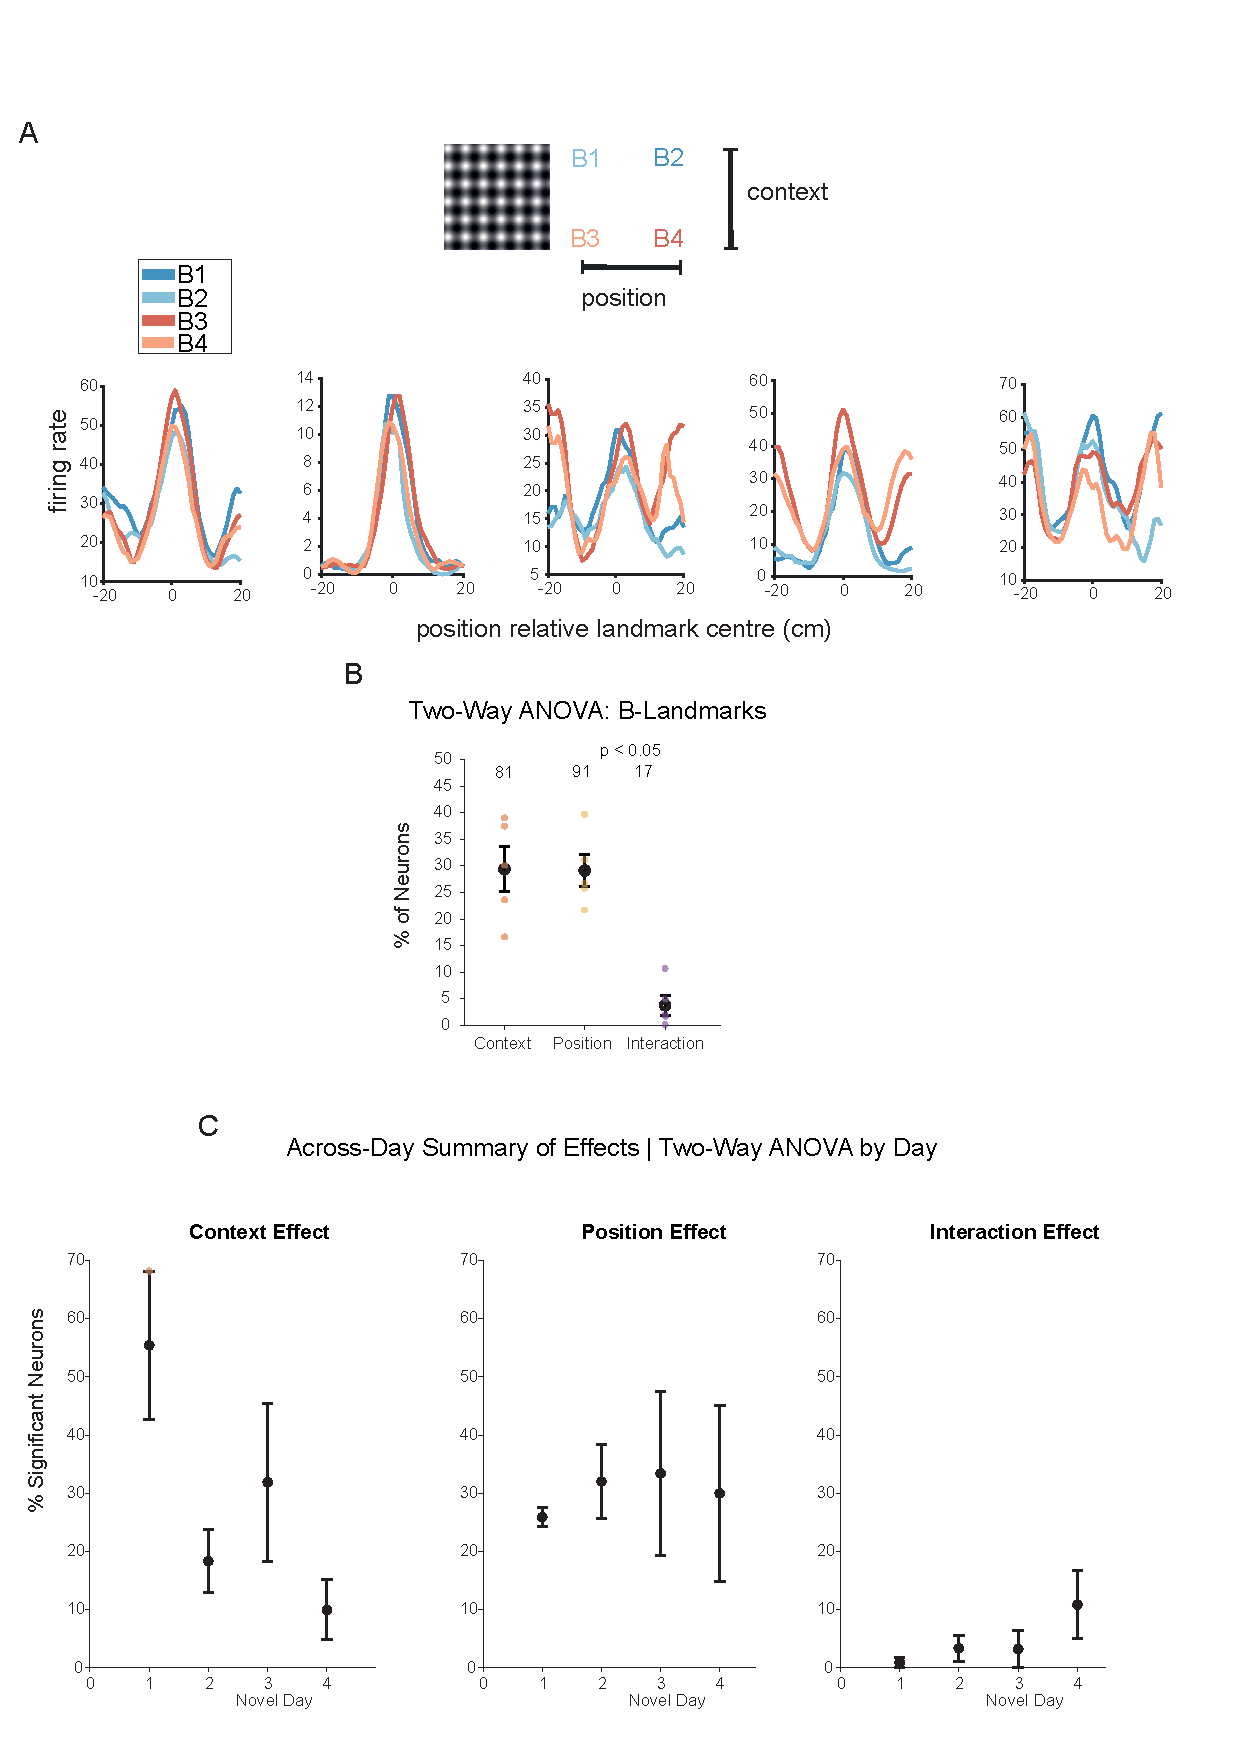
\includegraphics[width=1\linewidth]{figures//Chapter 4 V1/fig4_spatial_modulation_tests.pdf}
    \caption{Spatial and contextual modulations on landmarks shared by both environments. }
    \label{fig:placeholder}
\end{figure}